\section{Discussion}
\label{sec:discussion}

%To further explore the results of our
%experiment, we consider three issues:
%(1) a summary of the test path generation results
%obtained in this experiment and the practical implications,
%(2) a discussion of test input constraints, 
%and (3) a discussion of the security implications for our approach.
%Following this discussion, we address the limitations of our work. 
%
%\subsection{Test Path Generation Results and Practical Implications}
%
%Our results from the experiment strongly support the conclusion 
%that the program slice based test case generation approach needs 
%fewer test cases to test the modified version of the program 
%compared to the control technique.
%
%To show our results visually, we present them in bar graphs as shown
%in Figure~\ref{fig:bargraph}. The figure contains five subfigures 
%that present results for each object program, and each subfigure 
%contains bar graphs that show the total number of test paths produced 
%by two techniques (control (path-entire) and our technique (path-parte)).
%
%As the figure shows, for all version pairs of all object programs, 
%our approach generated a smaller number of test paths than the control 
%technique, and for the majority of the cases, the difference between 
%the control technique and our approach was very large. 
%In total, 12 of 20 version pairs produced over a 90\% reduction rate, for
%{\em Mambo} and {\em Mantis}, all cases but two produced substantial 
%reduction rates. 
%However, for some cases, the difference between these approaches was not 
%outstanding. For instance, with the first version pair in {\em osCommerce}, 
%the first two version pairs in {\em phpScheduleIt}, the second version pair 
%in {\em Mambo}, and the third version pair in {\em Mantis}, 
%the savings produced by our approach were smaller than average.
%We speculated that the version release affected this outcome. 
%When a software system goes through major version changes, 
%more functionalities tend to be added, and code refactoring can take 
%place; therefore, more code modifications are involved for the major revisions
%than for small bug fixes or feature updates.
%In fact, the version pairs that did not produce huge savings went through
%major changes, and large portions of code were refactored.
%
%The version pairs that produced substantial savings indeed involved
%minor bug fixes and small feature upgrades. 
%This is the exact situation where we aim to apply our approach
%as we described in the Introduction section. 
%Revisions caused by bug fixes or security problems tend to be unexpected 
%and unplanned compared to major revisions, thus a short turnaround time 
%for releasing these revisions is a dire issue. By providing regression testing 
%approaches that can save time and effort, we help deploy the applications
%as early as possible.
%
%\begin{figure*}[ht]
%%%\vspace*{-12pt}
%\centering
%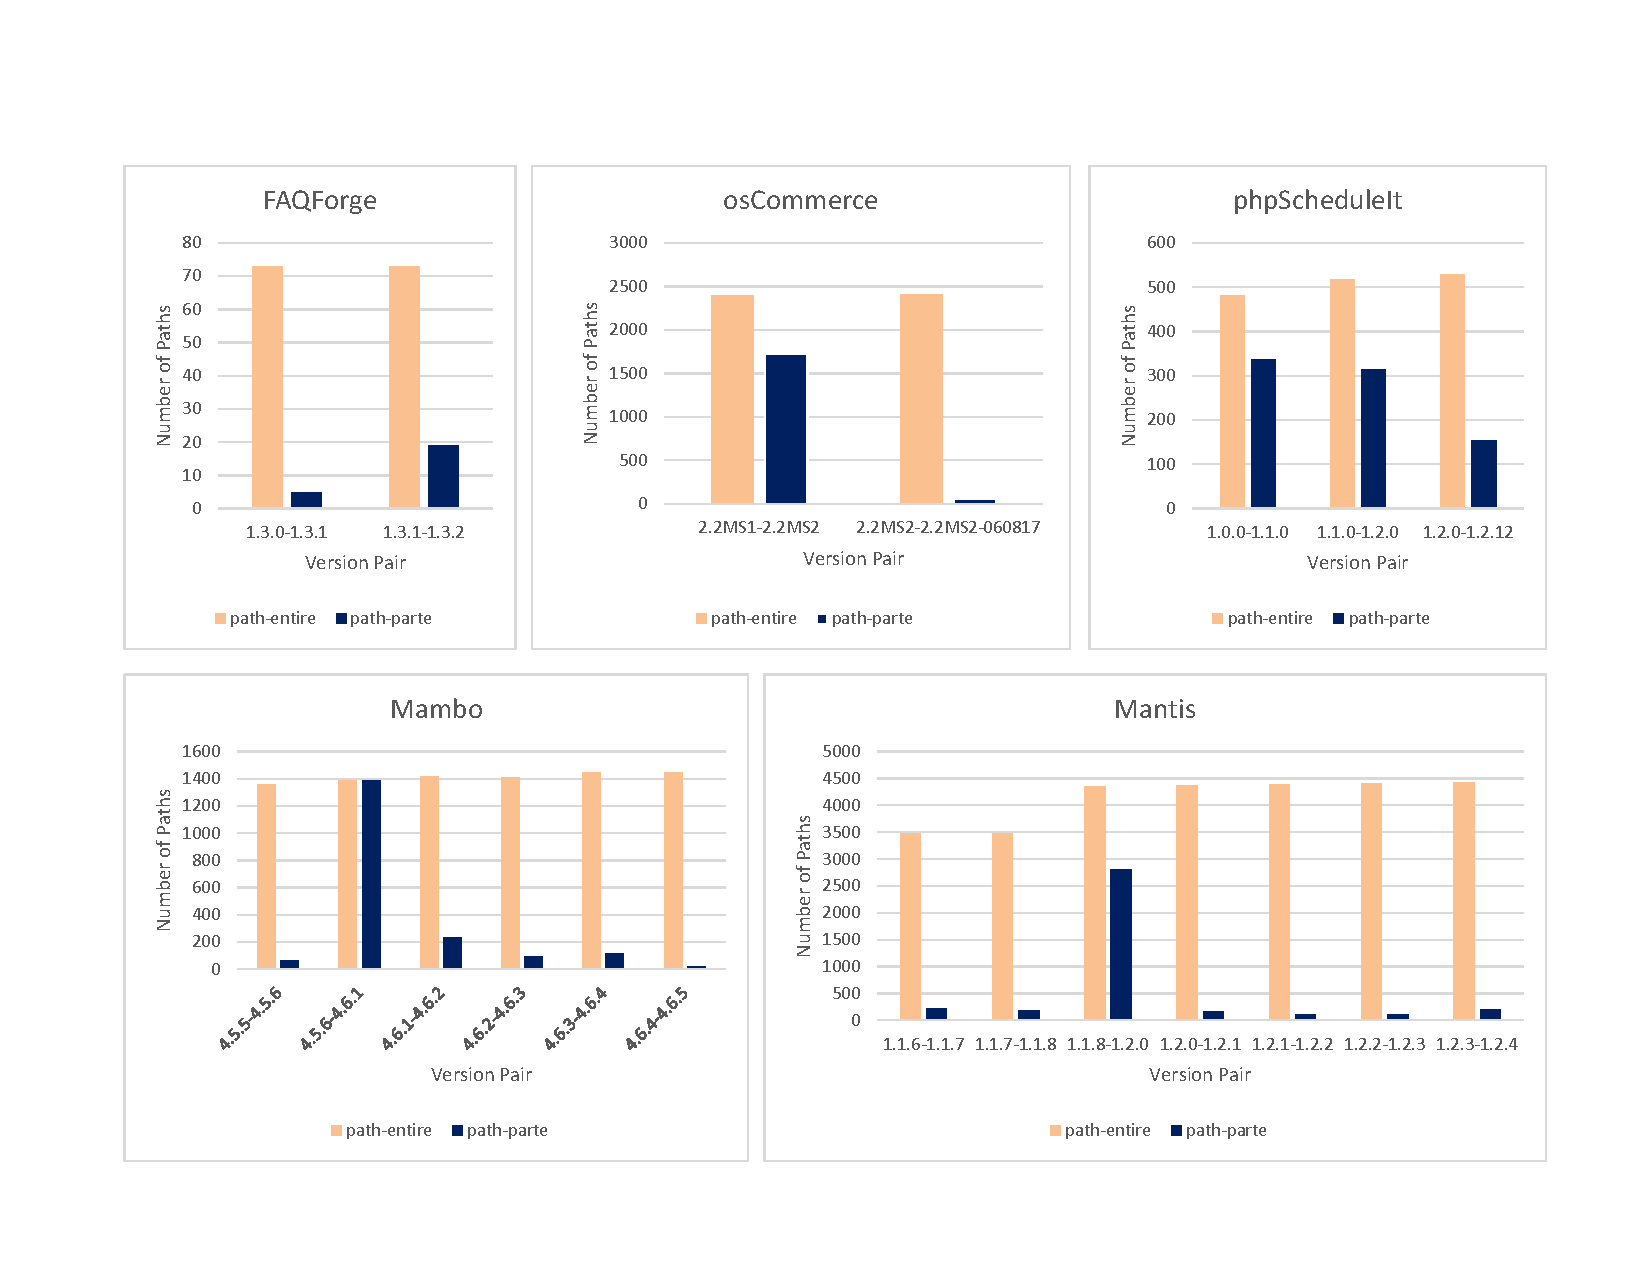
\includegraphics[width=1.0\columnwidth]{figures/bargraph.pdf}
%%\leavevmode \epsfxsize=1.0\columnwidth
%%\epsfbox{figures/bargraph.eps}
%\vspace*{-15pt}
%\caption{Experiment Results: The Total Number of Test Paths
%Generated by Control and PARTE techniques}
%\vspace*{5pt}
%\label{fig:bargraph}
%\vspace*{5pt}
%\end{figure*}
%
%\subsection{Test Input Constraints}
%
%Because the test paths require actual inputs to create executable
%test cases, by reducing the number of test paths necessary with the
%modified program, we expect to produce further savings for the costs
%associated with collecting test input constraints and resolving
%constraints.
%By automating the constraint resolution process for the majority
%of inputs, we could reduce a substantial amount of time and effort
%for resolving constraints manually.
%
%To provide some ideas about how much time we can save with automatic
%constraint resolution, we investigated the time taken to assign
%actual values to the input variables obtained by our constraint collector.
%We examined two cases from {\em osCommerce} that contain multiple numeric
%and string inputs. One case has 16 inputs (2 numeric and 14 string),
%and the other case has 10 inputs (2 numeric and 8 string).
%To resolve all input values, it took 15 and 20 minutes, 
%respectively. The tester had to go through the source files and the 
%application database to figure out the proper values for them.
%When we applied our tool, for the entire version of {\em osCommerce},
%it took less than 5 minutes.
%The input values assigned by human testers could be more realistic,
%but when the number of inputs is prohibitively large to be resolved 
%manually, automatic resolution would be the viable solution.
%Not all inputs can be resolved with the automatic resolution tool, but
%still, it would provide a good baseline that testers can utilize.
%
%\subsection{Security Implications}
%
%There are some security implications for this approach.
%Through the experiment, we observed that the applications we 
%used contained many security fixes and added security features,
%and we also observed that test cases generated with our approach 
%could help testers verify that a security patch or fix has been 
%properly implemented.
%
%In {\em FAQForge}, there was a security patch implemented 
%between versions 1.3.1 and 1.3.2. Our test generating tool 
%discovered the difference and generated several test cases 
%that traversed these changes. For version 1.3.1, changes 
%were made to the file that contains code for a login page that 
%allows the administrators to perform security associated tasks. 
%The change made to this file was the introduction of an HTML meta 
%tag with an http-equiv attribute. 
%This allows the page to load in all major browsers. Because the 
%change happens in the header, it is important to test all code 
%paths for the login page such as page load, validate username 
%and password, and count failed login attempts. The test paths generated 
%in our experiment include all these code paths or blocks.
%
%In {\em osCommerce}, a similar scenario occurred between versions
%2.2MS1 and 2.2MS2. The developers added some security features for 
%website administration. For example, features for supporting SSL 
%validation and forcing cookie usage were implemented.
%Another interesting security related feature was added to
%version 2.2MS2. This feature allowed users to inject shell commands 
%into the web server. Our tool generated several test cases that 
%covered this change. 
%However, without proper inputs for these test
%cases, we were not able to test this security feature correctly.
%Because our current constraint resolution tool does not generate 
%malicious inputs, we used our previous tool~\cite{marback09} to
%generate malicious inputs. With these inputs, our tool was able 
%to reveal this particular security vulnerability.
%In version 2.2MS2-060817, only a few minor security fixes were made. 
%For example, the fix prevented a session ID from being passed in 
%Tell-A-Friend E-Mails. This fix was a minor change to the statement 
%that prepares the body of the email to be sent. 
%Also, there was a security fix that corrected 
%an SQL injection problem between versions 2.2MS2 and 2.2MS2-060817. 
%Our tool was able to generate test cases
%that exercised all these fixes. 
%
%In the case of {\em phpScheduleIt}, version 1.2.0 introduced a security 
%feature where application administrators can grant permissions 
%to other users. These permissions provide users the access to make, 
%modify, or delete an existing reservation. Also, administrators can 
%remove permissions to prevent users from accessing a resource. 
%The regression tests for this version should cover code that was added 
%to enable user profile management. The results from our experiment show 
%that the new code blocks associated with new security features and fixes 
%were included in the regression test paths generated. 
%
%In version 4.6.2 of {\em Mambo}, a security fix was introduced. 
%One such fix is about the Captcha (completely automated public 
%turing test to tell computers and humans apart) feature. 
%If a session is not initiated, then it is regenerated, and a new 
%session code is assigned to the Captcha code. 
%This produces new challenge text and audio for verification. 
%Given the type and location of this fix it is important to cover all 
%viable paths in this code. All these code blocks were included 
%in the regression paths generated in our experiment.
% 
%In the case of {\em Mantis}, the version pair 1.1.6 and 1.1.7
%contained one security bug fix. The fix for this bug required 
%changes to the files that handle logging out of the current session 
%and reloading the verification page. 
%These changes impacted the blocks of code that perform logout, 
%initialize a new session, and validate user credentials.
%Another version pair, 1.1.8 and 1.2.0, contained one security fix. 
%The bug was about the possibility of a cross site scripting attack 
%through permalink\_page.php. The fix was to check if the input URL 
%is safe. Because this change happened at the root level, all paths 
%in the permalink\_page.php file should be included to test the fix,
%and our tool was able to generate those paths. 
% 
%\subsection{Limitations}
%\label{sec:limitations}
%
%Although our approach and empirical results are promising,
%our approach has some limitations that we want to address. 
%One limitation involves test oracles. As we mentioned
%in Section~\ref{sec:method}, in this work, we focused
%on generating test cases, and our approach does not generate
%the oracles. Automating test oracle generation or verification 
%of the results could be investigated in the future. 
% 
%Another limitation involves test case execution.
%To execute test cases automatically, the test execution engine 
%needs to pass the web elements to Selenium along with test paths and
%input values. However, the current path generator does not 
%provide web elements, so we had to provide them manually.
%As a result, we were not able to run all test cases that 
%we generated through our tool. However, this issue has been identified,
%and the feature addition is being developed. 
% 
